\chapter{Team Model}\label{chapter:team_model}

When evaluating players, it is very important to realize that the team they play for and their opponent will have a strong influence on their performance no matter the skill level.
\textit{Find something that states a player is directly affected by their team}

\section{Dixon and Coles}
Dixon and Coles set out to create a model that incorporates team's attacking and defending abilities \cite{dixon_coles}.

Dixon and Coles created a model with the aim of developing a profitable betting strategy for English football \cite{dixon_coles}.  The model assumes that the amount of goals scored by the home and away sides in any match are independent Poisson variables.  The means are determined by the attack and defence attributes of each side \cite{dixon_coles}.

Dixon and Robinson extended the previously discussed model by using the time each goal was scored instead of only the full time scores \cite{dixon_robinson}. 

\subsection{Model}

There are features 

\begin{itemize}
	\item The model should incorporate the different abilities of both teams.
	\item There should be an advantage for the team playing at home.
	\item The team abilities should be based on a summary of their recent games.
	\item A team's ability is likely to 
	\item When evaluating a team's performance, the ability of the opposing team should be taken into account.
	
\end{itemize}

The base assumption of the model is that the goals scored by the home and away teams are independent Poisson variables.  In a match between teams $i$ and $j$, the number of goals scored by the home and away teams are denoted by

$$X_{ij} ~ \text{Poisson}(\alpha_i\beta_j\gamma_h)$$
$$Y_{ij} ~ \text{Poisson}(\alpha_j\beta_i)$$

where $X_{ij}$ and $Y_{ij}$ are independent, $\alpha_i, \beta_i > 0.$

Dixon and Coles present the following to determine the probabilities of goals scored in a match.

\begin{equation}
\text{Pr}(X_{ij}=x, Y_{ij} = y) = \tau_{\lambda,\mu}(x, y)\frac{\lambda^x\exp(-\lambda)}{x!}\frac{\mu^y\exp(-\mu)}{y!}
\end{equation}

where

$$\lambda = \alpha_i\beta_j\gamma_h$$
$$\mu = \alpha_j\beta_i$$

and

\[
	\tau_{\lambda,\mu}(x,y) = 
	\begin{cases}
		1 - \lambda \mu \rho & \text{if } x=y=0,\\
		1 + \lambda \rho & \text{if } x=0,y=1,\\
		1 + \mu \rho & \text{if } x=1,y=0,\\
		1 - \rho & \text{if } x=1,y=1,\\
		1 & \text{otherwise}.
	\end{cases}
\]	

Dixon and Coles state that .  In the model, $\rho$ is a dependence parameter where $\rho=0$ corresponds to independence.  Basketball and football are fundamentally different sports, thus this dependence parameter is ignored for the basketball model.  

\subsection{Parameter Estimation}

From model \ref{eq:dc_likelihood} with $n$ teams, there are the attack abilities $\{\alpha_1,\ldots,\alpha_n\}$, defence abilities $\{\beta_1,\ldots,\beta_n\}$ and the home advantage parameter $\gamma$ to be estimated.  The constraint

$$\frac{1}{n}\sum_{i=1}^{n}\alpha_i = 1$$

is imposed by Dixon and Coles to keep the model from being over-parameterized.  For the basketball model, this constraint will be equal to 100 due to basketball scores being much higher than football.  

To estimate The National Basketball Association has 30 teams, thus the model has 61 parameters.  With matches indexed $k=1,\ldots,N$, and scores $(x_k, y_k)$, the likelihood function takes the form of



\begin{equation} \label{eq:dc_likelihood}
L(\alpha_i,\beta_i,\gamma, i=1,\ldots,n) = \prod_{k=1}^{N} \exp(-\lambda_k)\lambda_{k}^{x_k}\exp(-\mu_k)\mu_{k}^{y_k}
\end{equation}

where

$$\lambda_k = \alpha_{i(k)}\beta_{j(k)}\gamma,$$
$$\mu_k = \alpha_{j(k)}\beta_{i(k)}$$

The team abilities for the NBA can be seen in Table \ref{table:dc_141516}.  Using these numbers, and selecting the team with the highest probability of winning a game.  The accuracy of selecting a winner was 63.84\% and the value betting strategy won 57.84 units with 37.06\% winning bets.




\subsection{Model Limitation and Modification}

The main limitation of model \ref{eq:dc_likelihood} is that the parameters are static.  The team abilities are constant throughout time, when in reality they are always evolving.  Since we are always estimating team parameters at a certain time point $t$, Dixon and Coles proposed that more recent matches should hold higher value compared to it's historical counterparts.  Adjusting equation \ref{eq:dc_likelihood} leads to

\begin{equation} \label{eq:dc_likelihood_time}
L(\alpha_i,\beta_i,\gamma, i=1,\ldots,n) = \prod_{k=1}^{N} \left\lbrace \exp(-\lambda_k)\lambda_{k}^{x_k}\exp(-\mu_k)\mu_{k}^{y_k}\right\rbrace ^{\phi(t-t_k)}
\end{equation}

where $t$ is the time the estimation is made, $t_k$ is the time match $k$ was played and $\phi$ is a non-increasing function of time.


They chose the model to be

$$\phi(t) = \exp(-\xi t)$$

\begin{equation}
	L(\alpha, \beta) = \left\lbrace \exp(-\lambda_k) \lambda_{k}^{x_k}\exp(-\mu_{k})\mu_k^{y_k}\right\rbrace^{\phi(t-t_k)} 
\end{equation}

\begin{equation} \label{eq:home_prob}
	p_k^H = \sum \text{Pr}(X_k = x, Y_k = y) 
\end{equation}

\begin{equation} \label{eq:s_estimation}
	S(\xi) = \sum_{k=1}^{N}(\delta_k^H\log p_k^H + \delta_k^A\log p_k^A + \delta_k^D\log p_k^D)
\end{equation}

\begin{figure}[ht]
	\centering
	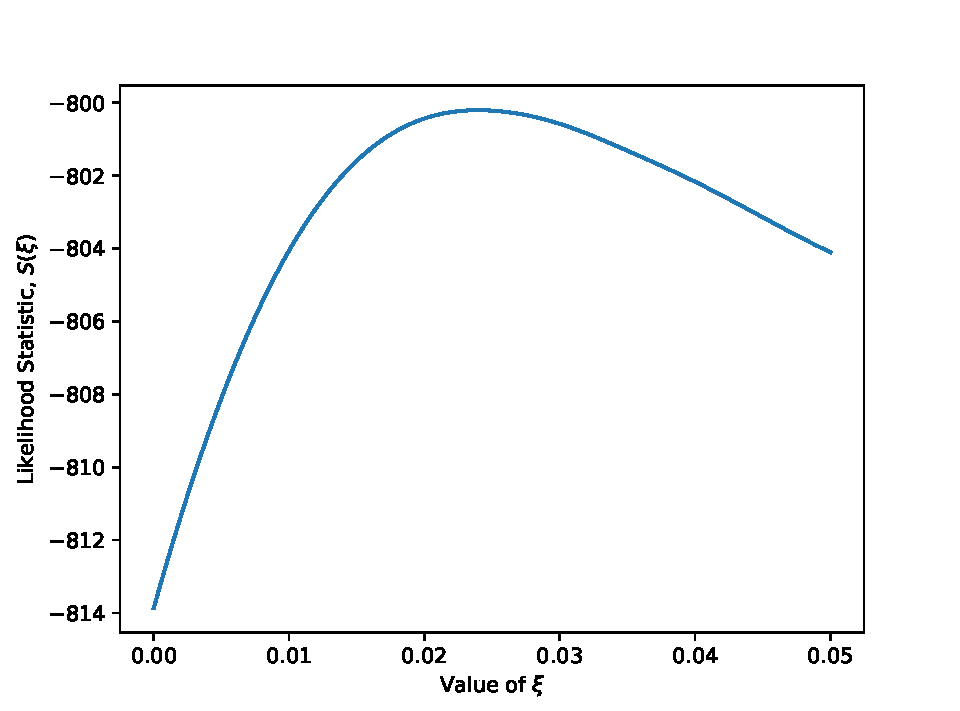
\includegraphics[width=1\textwidth]{{Figures/xi_plot.pdf}}
	\captionof{figure}{S($\xi$) vs $\xi$: The maximum occurs at $\xi = 0.024$.}
	\label{fig:play_by_play}
\end{figure}

\begin{figure}[ht]
	\centering
	\begin{subfigure}{0.67\linewidth}
	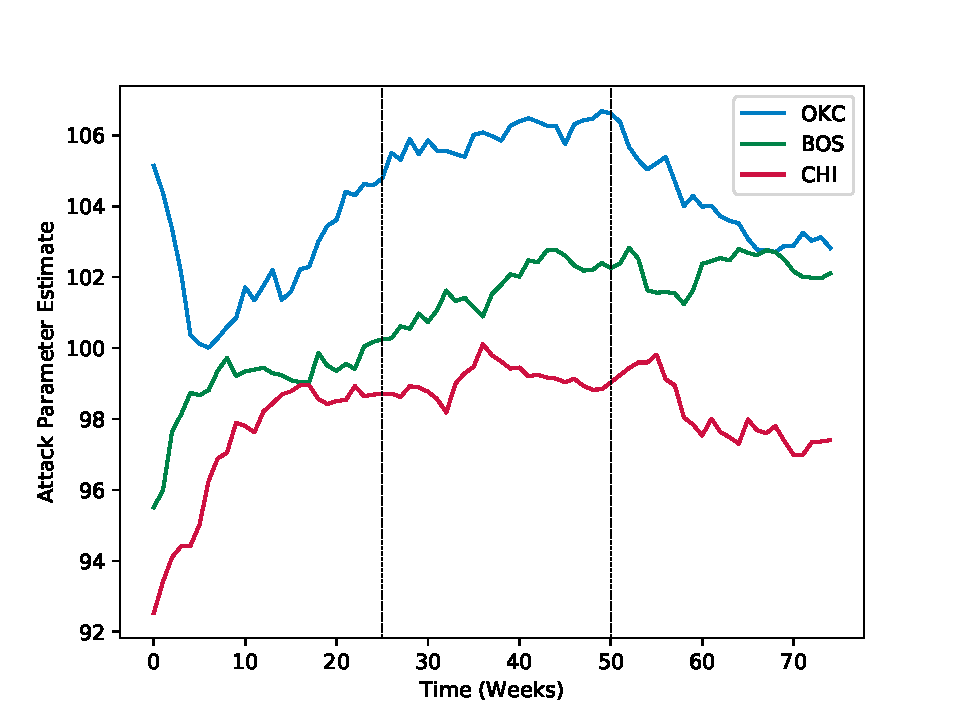
\includegraphics[width=1\textwidth]{{Figures/weeks_attack.pdf}}
	\caption{}	
	\end{subfigure}
	
	\begin{subfigure}{0.67\linewidth}
	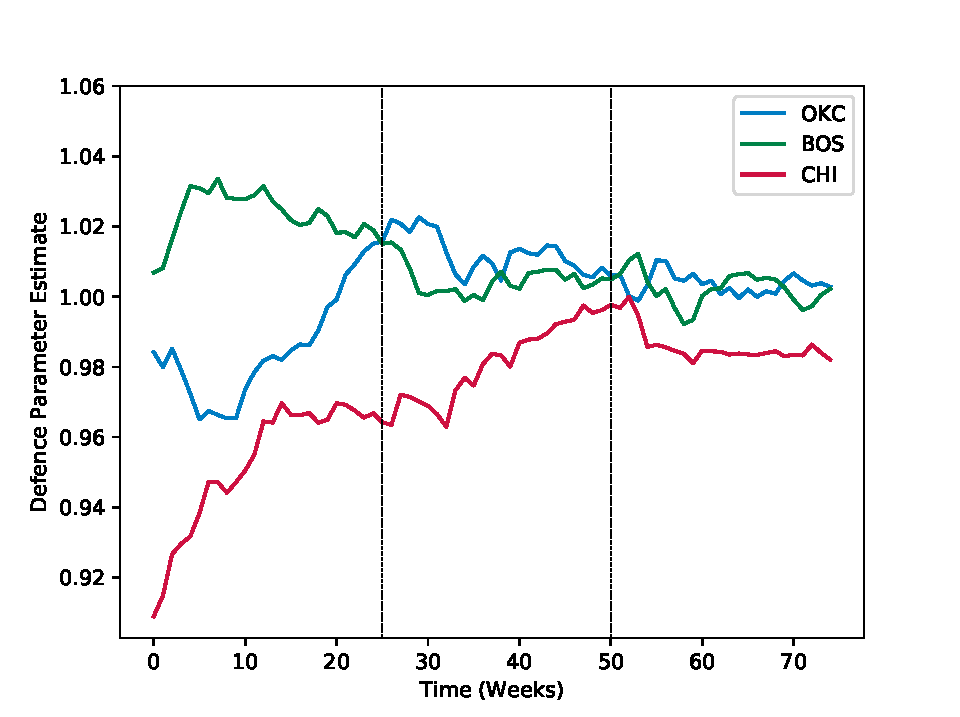
\includegraphics[width=1\textwidth]{{Figures/weeks_defence.pdf}}
	\caption{}
	\end{subfigure}
	
	\begin{subfigure}{0.67\linewidth}
	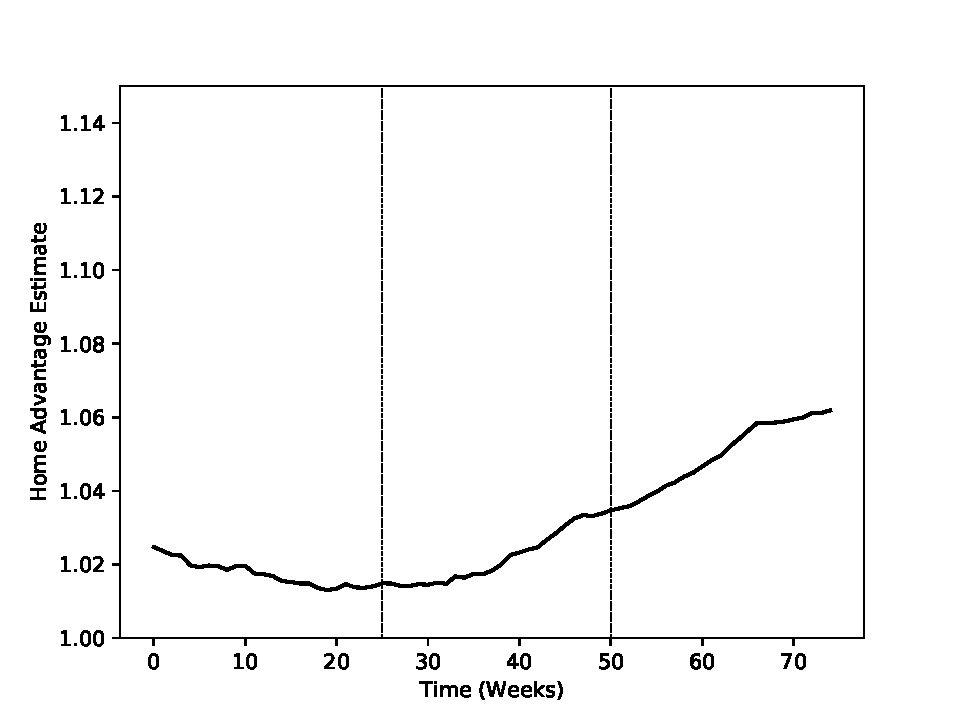
\includegraphics[width=1\textwidth]{{Figures/weeks_home.pdf}}
	\caption{}
	\end{subfigure}
	
	\caption{(A),(B) Attack and defence parameter weekly estimates for the Oklahoma City Thunder, Boston Celtics and Chicago Bulls; (C) Home advantage parameter variation.}
	\label{fig:weeks_dc}
	
\end{figure}